\documentclass{beamer}

\usetheme{custom}
\usepackage{amsmath, amssymb}

% Language formatting
\usepackage[utf8]{inputenc}
\usepackage[T1]{fontenc}
\usepackage[spanish, es-noshorthands]{babel}

% Graph and Drawings
\usepackage{tikz,float}
\usetikzlibrary{babel}
\usetikzlibrary{backgrounds}
\usetikzlibrary{arrows.meta}
\usetikzlibrary{positioning}

% Tools
\usepackage{ragged2e} 
\usepackage{hyperref}
\usepackage{etoolbox,mathtools}
\usepackage[shortlabels]{enumitem}
\usepackage{array} 
\usepackage[noend]{algpseudocode}
\usepackage{algpseudocodex}

% Resize abs and norm
\DeclarePairedDelimiter{\abs}{\lvert}{\rvert}
\DeclarePairedDelimiter{\norm}{\|}{\|}
\makeatletter
\let\oldabs\abs
\def\abs{\@ifstar{\oldabs}{\oldabs*}}
\let\oldnorm\norm
\def\norm{\@ifstar{\oldnorm}{\oldnorm*}}
\makeatother

% Symbols

\newcommand{\N}{\mathbb{N}}
\newcommand{\R}{\mathbb{R}}

\newcommand{\PP}{\mathcal{P}}
\newcommand{\TT}{\mathcal{T}}
\newcommand{\KK}{\mathcal{K}}
\newcommand{\RR}{\mathcal{R}}
\newcommand{\OO}{\mathcal{O}}

\DeclareMathOperator{\separation}{separation}
\DeclareMathOperator{\reach}{reach}
\DeclareMathOperator{\height}{height}
\DeclareMathOperator{\angularDev}{angularDeviation}
\DeclareMathOperator{\centre}{center}
\DeclareMathOperator{\setint}{int}
\DeclareMathOperator{\Delloc}{Delloc}
\DeclareMathOperator{\medialAxis}{medialAxis}
\DeclareMathOperator{\vertex}{vert}
\DeclareMathOperator{\diam}{diam}
\DeclareMathOperator{\VR}{VR}
\DeclareMathOperator{\Cech}{\check{C}}
\DeclareMathOperator{\relint}{relint}
\DeclareMathOperator{\conv}{conv}
\DeclareMathOperator{\aff}{aff}
\DeclareMathOperator{\Del}{Del}
\DeclareMathOperator{\nerve}{nerve}
\DeclareMathOperator{\card}{card}
\DeclareMathOperator{\dist}{dist}

\definecolor{edgeColor}{rgb}{0.5,0.1,0.05}
\definecolor{mybg}{rgb}{1.0,0.99,0.82}

\tikzset{
  myvertex/.style={fill=black, circle, inner sep=0pt, outer sep=0pt, minimum size=3pt},
  myedge/.style={color=edgeColor,line width=1.5pt}
}

\setlength{\fboxsep}{0pt}%
\setlength{\fboxrule}{1pt}%

\newenvironment{Algoritmo}%
{ \begin{figure}[H]
  \centering
  \begin{algorithmic}[1]}
{\end{algorithmic}\end{figure} }

\title[Reconstrucción de Superficies]{Reconstrucción de Superficies por Nube de Puntos}
\author{Sebastián Sánchez}
\date{2023}

\AtBeginSection[]
{%
  \begin{frame}
    \frametitle{Tabla de Contenidos}
    \tableofcontents[currentsection]
  \end{frame}
}

\begin{document}

\frame{\titlepage}

%%%%%%%%%%%%%%%%%%%%%%%%%%%%%%%%%%%%%%%%%%%%%%%%%%%%%%%%%%%%%%%%%
\section{Introducción}

\begin{frame}\frametitle{Introducción}
  Dada una muestra finita de puntos \(P\) en \(\R^N\) que viven sobre
  una superficie \(M\subset\R^N\):
  \begin{itemize}
    \item ¿Es posible reconstruir la superficie?
    \item ¿Qué entendemos por reconstruir?
    \item ¿Qué tipo de superficies y bajo qué condiciones?
  \end{itemize}
\end{frame}

%  \begin{block}{Notación}
%  \(X^{\oplus \epsilon} \coloneqq \lbrace y\in\R^N \colon d(y,X) < \epsilon \rbrace\)
%  \end{block}

\begin{frame}\frametitle{Ambigüedades}
  \usetikzlibrary[plotmarks]
  \begin{figure}[H]
  \begin{overprint}
  \onslide<1>
  \centering
  \begin{tikzpicture}[framed, scale=2]
    \draw[only marks, mark=*, mark size=1pt, domain=0:360, samples=20, variable=\t] 
      plot (\t:{1-.8*cos(4*\t)});
  \end{tikzpicture}
  \onslide<2>
  \centering
  \begin{tikzpicture}[framed, scale=2]
    \draw[only marks, mark=*, mark size=1pt, domain=0:360, samples=100, variable=\t] 
      plot (\t:{1-.8*cos(4*\t)});
  \end{tikzpicture}
  \end{overprint}
  \end{figure}

  \begin{Definicion}[Muestra Densa y Ruidosa]
    \(P\) es \(\epsilon\)-densa si \(M\subset P^{\oplus \epsilon}\)
    y \(\delta\)-ruidosa si \(P\subset M^{\oplus \delta}\).  
  \end{Definicion}
\end{frame}

\begin{frame}\frametitle{¿Qué entendemos por reconstruir?}
  \begin{overprint}
    \onslide<1>\centering\fbox{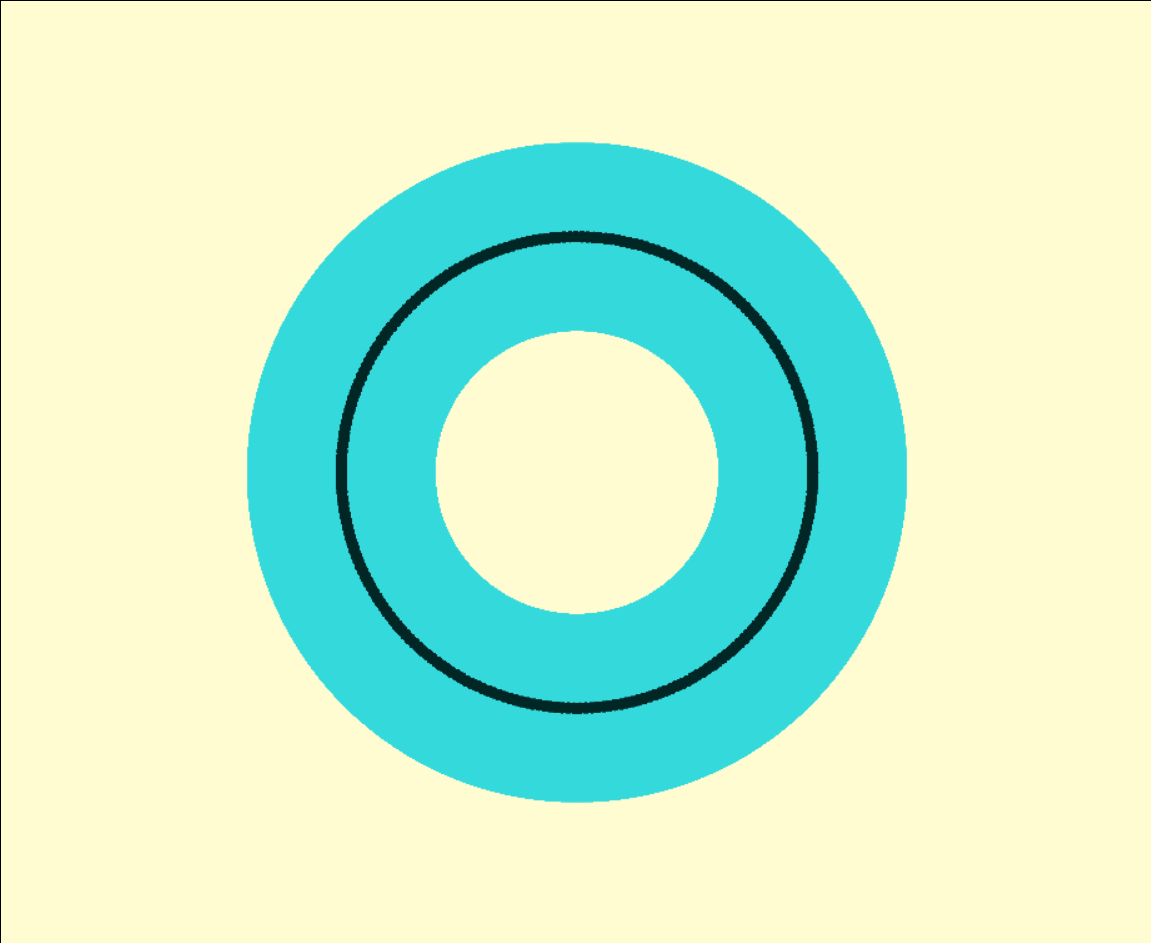
\includegraphics[height=.7\textheight]{slidesRes/reconst1.png}}
    \onslide<2>\centering\fbox{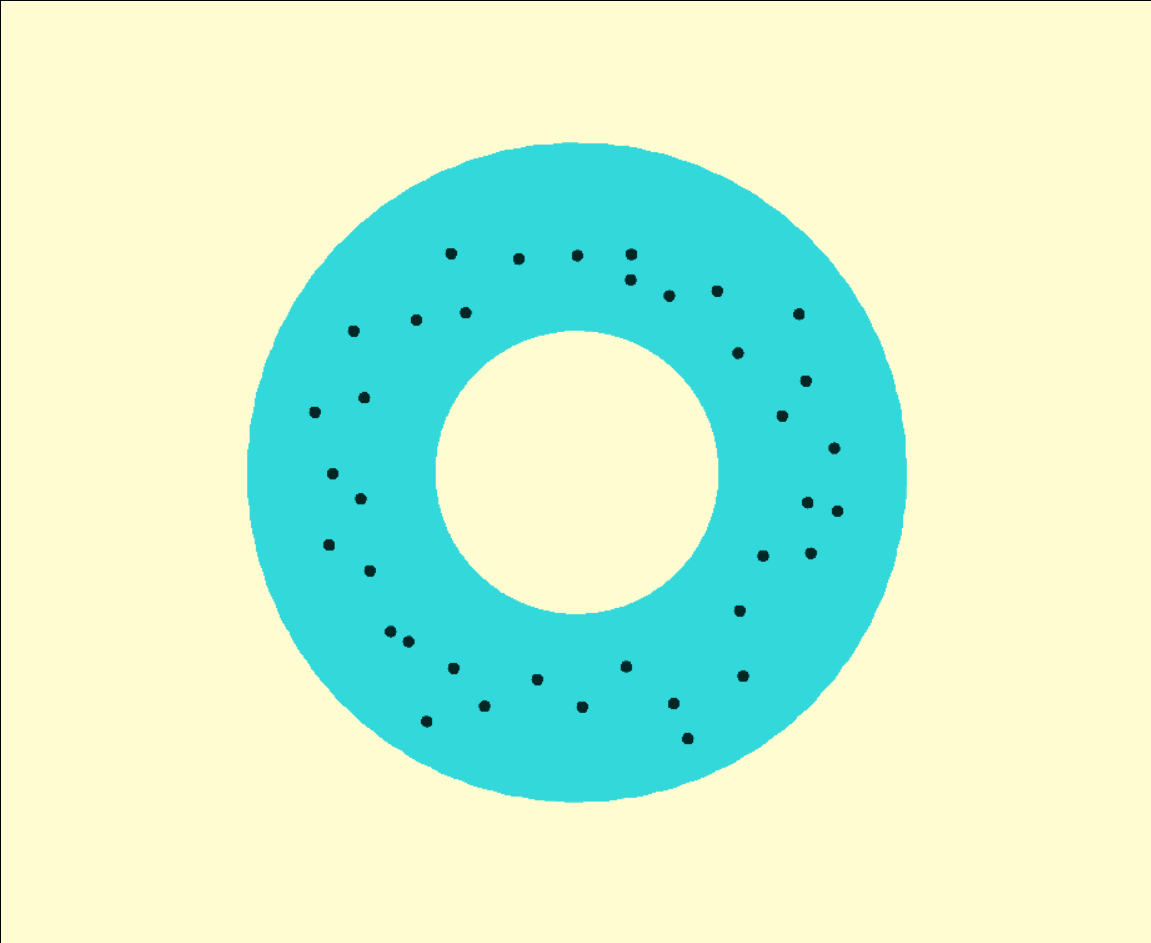
\includegraphics[height=.7\textheight]{slidesRes/reconst3.png}}
    \onslide<3>\centering\fbox{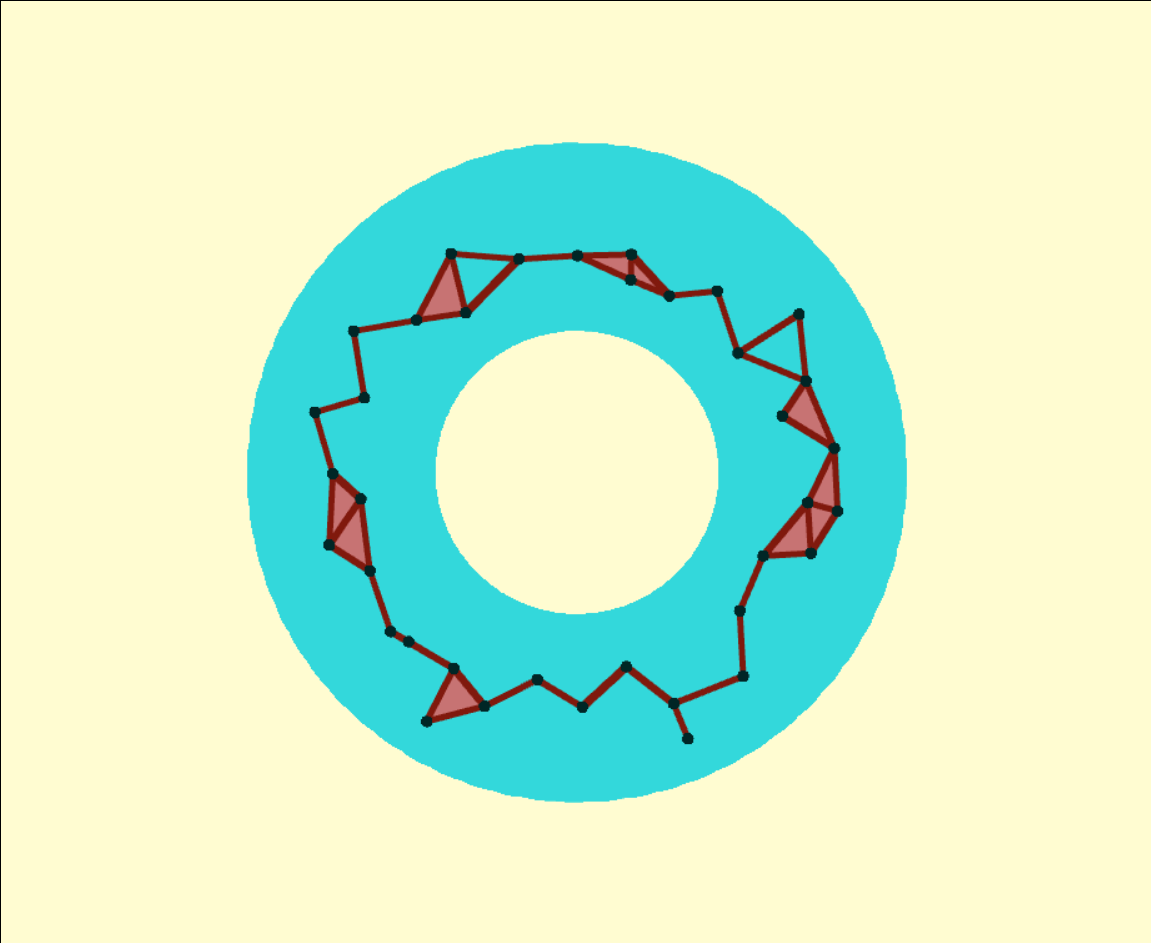
\includegraphics[height=.7\textheight]{slidesRes/reconst2.png}}
  \end{overprint}
\end{frame}

\begin{frame}\frametitle{Complejos Simpliciales}
Un símplice es la generalización de un triángulo.

\begin{figure}[htpb]
\centering\fbox{\begin{tikzpicture}[framed, background rectangle/.style={fill=mybg}, show background rectangle]
\begin{scope}
  \node[myvertex] (00) at (0,0){}; 
  \node[myvertex] (11) at (1,1){}; 
  \draw[myedge] (00) -- (11);
\end{scope}

\begin{scope}[xshift=2cm]
  \node[myvertex] (00) at (0,0){}; 
  \node[myvertex] (01) at (0,1){}; 
  \node[myvertex] (10) at (1,0){}; 
  \draw[myedge] (00) -- (01) -- (10) -- (00);
\end{scope}

\begin{scope}[xshift=4cm]
  \node[myvertex] (000) at (0,0,0){}; 
  \node[myvertex] (001) at (0,0,1){}; 
  \node[myvertex] (010) at (0,1,0){}; 
  \node[myvertex] (100) at (1,0,0){}; 
  \draw[myedge] (000) -- (001) -- (010) -- (000);
  \draw[myedge] (000) -- (001) -- (100) -- (000);
  \draw[myedge] (000) -- (010) -- (100) -- (000);
\end{scope}
\end{tikzpicture}}
\end{figure}

Y un complejo simplicial es la generalización de una triangulación.
\begin{figure}[H]
  \centering
  \fbox{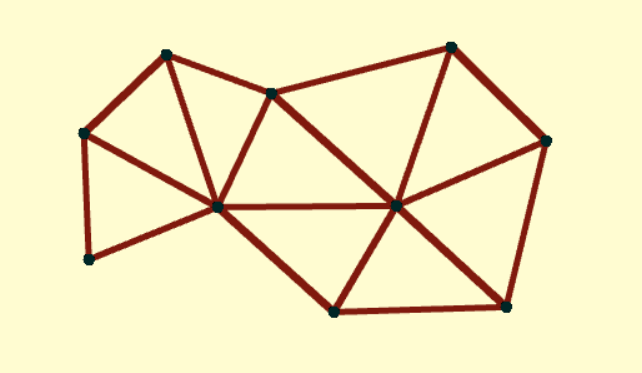
\includegraphics[width=.4\textwidth]{slidesRes/triangulation.png}}
\end{figure}
\end{frame}


\begin{frame}\frametitle{¿Qué entendemos por reconstruir?}
  \begin{Definicion}[Reconstrucción Fidedigna]
    Un complejo simplicial \(K\) con conjunto de vértices en \(P\subset \R^N\)
    reconstruye a un espacio \(X\subset\R^N\) de manera fidedigna si 
    \begin{enumerate}
      \item \(K\) es geometricamente realizable.
      \item \(\bigcup K \coloneqq \bigcup_{\sigma \in K} \conv \sigma\) está contenido en
        una región tubular de \(X\).
      \item La proyección de \(\bigcup K\) a \(X\) es un homeomorfismo.
    \end{enumerate}
  \end{Definicion}
  \pause%
  De ahora en adelante \(M\) es una \(d\)-subvariedad de \(\R^N\) (con o sin borde) compacta, orientable, 
  suave y \(P\) es una muestra \(\epsilon\)-densa
  \(\delta\)-ruidosa de \(M\).
\end{frame}

\begin{frame}\frametitle{¿Qué entendemos por reconstruir?}
  \begin{figure}[H]
    \centering\fbox{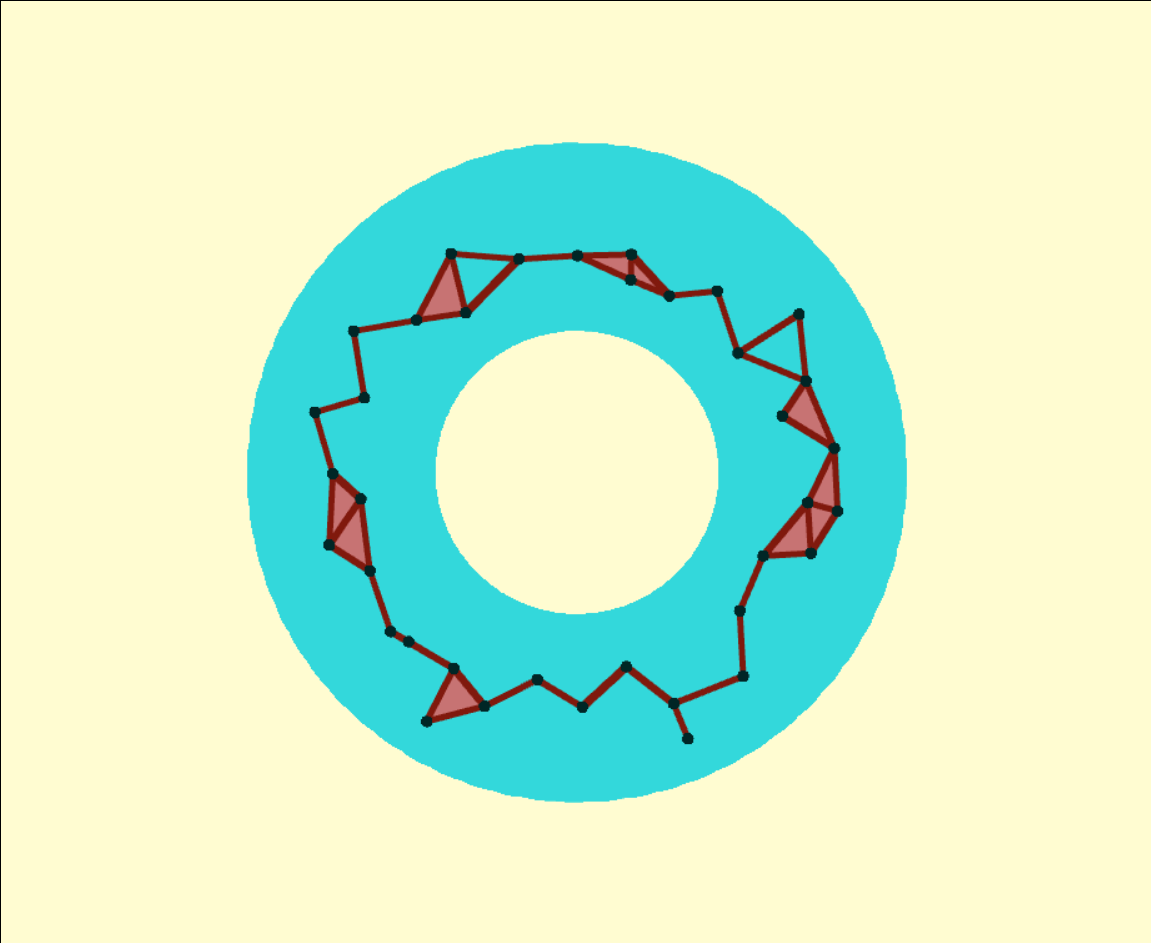
\includegraphics[height=.7\textheight]{slidesRes/reconst2.png}}
    \caption{No es una reconstrucción fidedigna.}
  \end{figure}
\end{frame}

%\begin{frame}\frametitle{Complejos Simpliciales}
%Un \(d\)-símplice geométrico es la cáscara convexa de \(d+1\) puntos
%afínmente independientes. Una cara de un \(d\)-símplice \(\sigma\) es un \(k\)-símplice
%formado por \(k+1\) puntos que definen \(\sigma\). 
%
%\begin{figure}[H]
%\begin{center}
%\begin{tikzpicture}[black,framed]
%  \begin{scope}
%    \node[myvertex] (A) at (0,0) {};
%    \node[myvertex] (B) at (1,-1) {};
%    \node[myvertex] (C) at (1,1) {};
%    \draw[myedge] (A) -- (B) -- (C) -- (A);
%  \end{scope}
%  \begin{scope}[xshift=2cm]
%    \node[myvertex] (A) at (0,0) {};
%    \node[myvertex] (B) at (1,-1) {};
%    \node[myvertex] (C) at (1,1) {};
%    \node[myvertex] (D) at (0,1) {};
%    \draw[myedge] (A) -- (B) -- (C) -- (A);
%    \draw[myedge] (A) -- (D);
%  \end{scope}
%  \begin{scope}[xshift=4cm]
%    \node[myvertex] (A) at (0,0) {};
%    \node[myvertex] (B) at (1,-1) {};
%    \node[myvertex] (C) at (1,1) {};
%    \node[myvertex] (D) at (2,0) {};
%    \draw[myedge] (A) -- (B) -- (C) -- (A);
%    \draw[myedge] (A) -- (D);
%  \end{scope}
%\end{tikzpicture}
%\end{center}
%\end{figure}
%
%Un complejo simplicial geométrico es una colección de símplices
%que es cerrada bajo intersección y contiene todas las caras de sus elementos.
%\end{frame}

%%%%%%%%%%%%%%%%%%%%%%%%%%%%%%%%%%%%%%%%%%%%%%%%%%%%%%%%%%%%%%%%%
\section{Complejos Simpliciales}

\begin{frame}\frametitle{¿Cómo construir complejos?}
  \begin{itemize}[itemsep=2em]
    \item<1-> Queremos unir los puntos considerando su cercanía
    \item<2-> Idea natural: considerar bolas centradas en los puntos de muestra
  \end{itemize}
\end{frame}


%\begin{frame}\frametitle{Evitar malos casos}
%\begin{Definicion}[Posición general]
%  Decimos que un conjunto \(P\subset\R^N\) está en posición general si 
%  no hay \(N+2\) puntos coesféricos y todo subconjunto \(Q\subset P\)
%  de tamaño menor a \(N+1\) es afínmente independiente. 
%\end{Definicion}
%
%\begin{itemize}
%  \item En \(\R^2\): no hay \(4\) puntos en un círculo ni hay \(3\) puntos colineales.   
%  \item En \(\R^3\): no hay \(5\) puntos en una esfera ni hay \(4\) puntos coplanares ni
%  \(3\) puntos colineales.   
%\end{itemize}
%
%De aquí en adelante supondremos que \(P\) está en posición general. 
%\end{frame}
%
\subsection{Complejo de Delaunay}
%
%\begin{frame}\frametitle{Complejo de Delaunay}
%\begin{center}
%{
%\setlength{\fboxsep}{5pt}%
%\setlength{\fboxrule}{1pt}%
%\fbox{
%\begin{tikzpicture}[scale=4, transform shape, myedge/.style={color=edgeColor, line width=1.5pt}]
%  \node[myvertex] (A) at (0,-.1) {};
%  \node[myvertex] (B) at (.5,1) {};
%  \node[myvertex] (C) at (1.2,-.2) {};
%  \node[myvertex] (D) at (.9,0.7) {};
%  \node[myvertex] (E) at (1.2,.8) {};
%  \node[myvertex] (F) at (.7,0.2) {};
%
%  \onslide<2->
%  \draw[myedge] (A) -- (B);
%  \draw[myedge] (A) -- (F);
%  \draw[myedge] (A) -- (C);
%
%  \onslide<3->
%  \draw[myedge] (B) -- (F);
%  \draw[myedge] (B) -- (D);
%  \draw[myedge] (B) -- (E);
%
%  \onslide<4->
%  \draw[myedge] (D) -- (F);
%  \draw[myedge] (D) -- (E);
%  \draw[myedge] (D) -- (C);
%  
%  \onslide<5->
%  \draw[myedge] (F) -- (C);
%  \draw[myedge] (E) -- (C);
%\end{tikzpicture}
%}}
%\end{center}
%\end{frame}

\begin{frame}\frametitle{Voronoi}
\begin{columns}
  \column{.6\linewidth}
  \begin{itemize}[itemsep=1em]
    \item<1->
    Una celda Voronoi \(V_p\) consiste en los puntos que están más cercanos a \(p\) que
    a cualquier otro punto \(q\) de \(P\).
    \begin{equation*}
      V_p \coloneqq \left\{ x\in \R^N \colon \abs{xp} \le \abs{xq}\quad \forall q\ne p \right\}.
    \end{equation*}

    \item<2->
    El diagrama de Voronoi de un conjunto de puntos, \(V_P\), es la colección de celdas
    de Voronoi de sus elementos.
    \begin{equation*}
      V_P \coloneqq \left\{ V_p \colon p\in P \right\}.
    \end{equation*}
  \end{itemize}

  \column{.4\linewidth}
  \begin{figure}[H]
    \begin{overprint}
      \onslide<1>\centering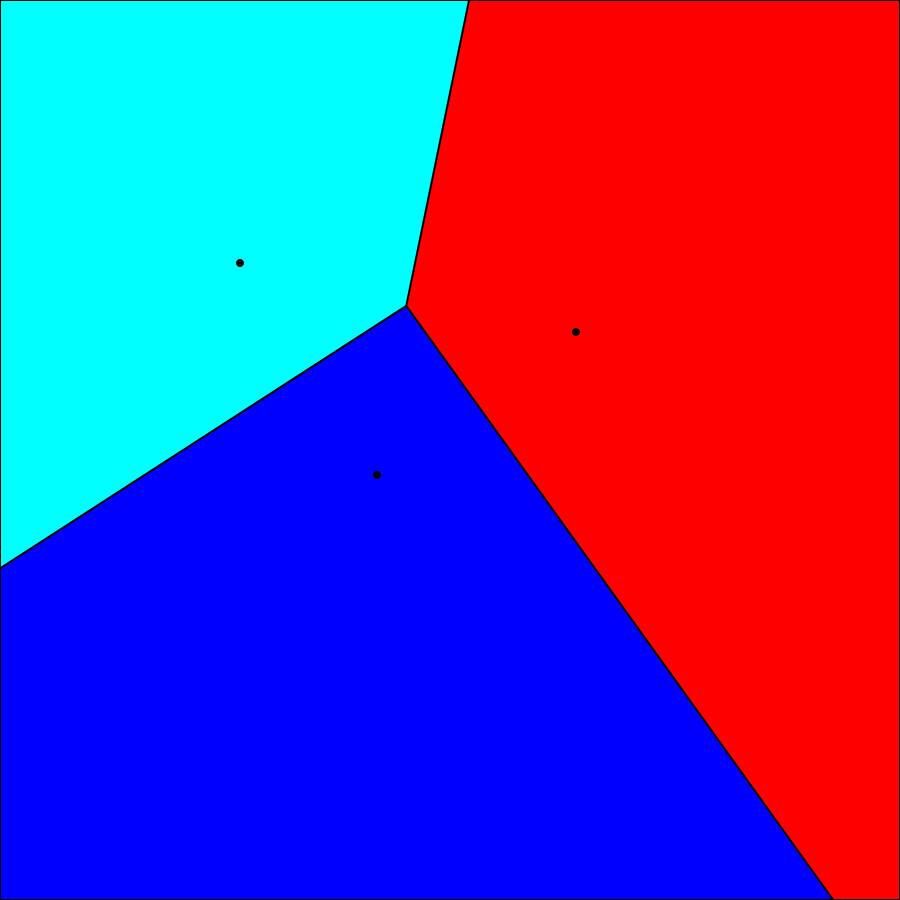
\includegraphics[width=\textwidth]{slidesRes/voronoi.png}
      \caption{Diagrama de Voronoi de 3 puntos en el plano.}
      \onslide<2>\centering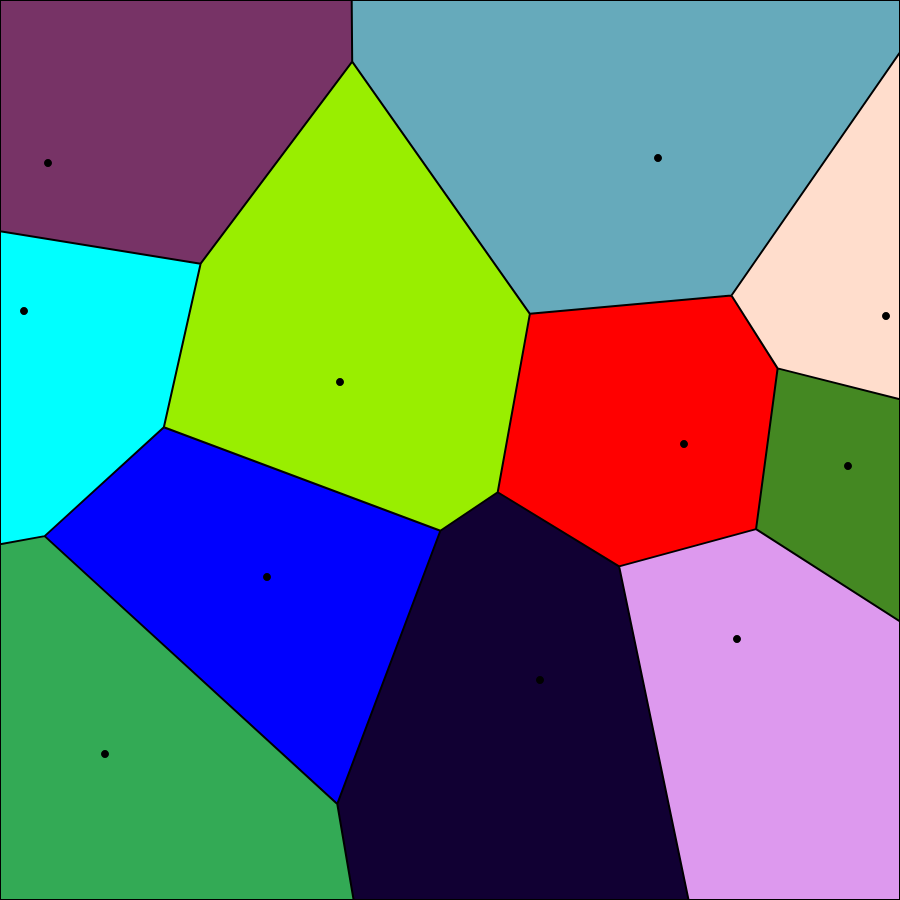
\includegraphics[width=\textwidth]{slidesRes/voronoi10.png}
      \caption{Diagrama de Voronoi de 10 puntos en el plano.}
    \end{overprint}
  \end{figure}
\end{columns}
\end{frame}

%\begin{frame}\frametitle{Complejo de Delaunay}
%\begin{Definicion}[Complejo de Delaunay]
%  \(Q\subset P\) es un símplice de Delaunay si existe una bola
%  abierta \(B\) tal que \(Q\subset \partial B\) y \(B\cap P = \varnothing\).
%  El complejo de Delaunay asociado a \(P\) es:
%  \(
%    \Del(P) \coloneqq \left\{ Q\subset P \colon Q \text{ es un símplice de Delaunay} \right\}.
%  \) 
%\end{Definicion}
%\end{frame}

\begin{frame}\frametitle{Complejo de Delaunay}
  \begin{Definicion}[Complejo de Delaunay]
  \begin{displaymath}
    \Del(P) = \lbrace Q\subset P \colon \bigcap_{p\in Q} V_p \ne \varnothing \rbrace
  \end{displaymath}
  \end{Definicion}
\begin{figure}[H]
\begin{columns}
  \column{.7\textwidth}
  \centering\fbox{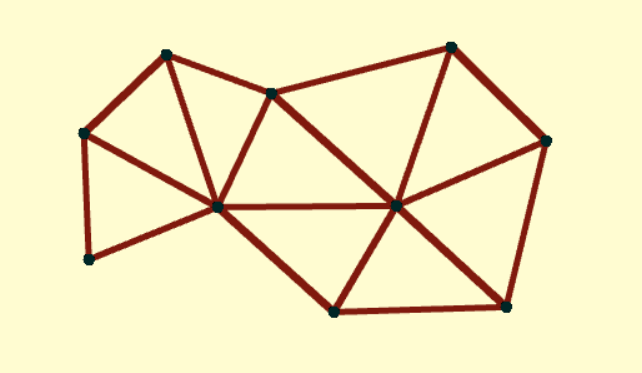
\includegraphics[height=.5\textheight]{slidesRes/triangulation.png}}
  \column{.3\textwidth}
  \caption{\small No es un complejo de Delaunay.}
\end{columns}
\end{figure}
\end{frame}
%\begin{frame}\frametitle{Observaciones}
%\begin{columns}
%  \column{.5\linewidth}
%  \begin{itemize}
%    \item<1-> Cada región \(V_p\) es un polihedro convexo. 
%    \item<2-> Dado \(N+1\) puntos \(Q = \left\{ q_0,\ldots,q_N\right\}\), 
%    se tiene que \(\bigcap_{q\in Q} V_q\) es un único punto o vacía.  
%    \item<3-> En particular, la intersección de \(N+2\) regiones
%    siempre es vacía.
%  \end{itemize}
%  \column{0.5\linewidth}
%  \begin{figure}[H]
%    \centering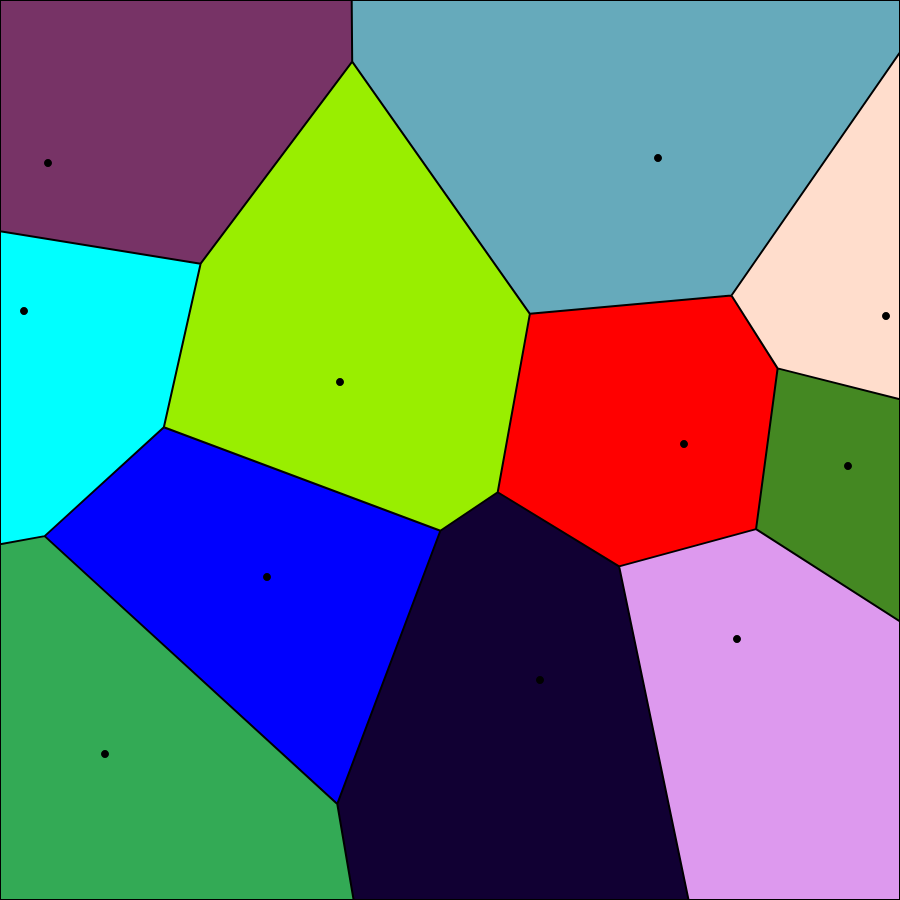
\includegraphics[width=\textwidth]{slidesRes/voronoi10.png}
%    \caption{Diagrama de Voronoi de 10 puntos en el plano.}
%  \end{figure}
%\end{columns}
%\end{frame}


%\begin{frame}
%\begin{Teorema}
%  \(\Del(P)\) reconstruye de manera fidedigna a \(\conv P\).
%\end{Teorema}
%
%\begin{proof}
%  (\(\Rightarrow\):) \(x\in \bigcup \Del(P) \Rightarrow x\in \conv Q \Rightarrow x\in \conv P\).  
%
%  (\(\Leftarrow\):) \(x\in \conv P\). 
%  \begin{itemize}
%    \item Caso 1: \(\card P \le N+1\):  \(\Rightarrow P\in\Del(P)\).
%    \item Caso 2: \(\card P > N+1\): Tomar \(Q = \lbrace P_1, \ldots, P_N \rbrace\) los \(N\) 
%    puntos más cercanos a \(x\). Notar \(B_N \cap P \subset Q\). Sea
%    \(P_{N+1}\) el siguiente punto más lejano a \(x\). 
%    Luego, \(x\in \conv (P_1, \dots, P_{N+1})\) y existe una única
%    esfera que circumscribe a \(P_1, \dots, P_{N+1}\). 
%  \end{itemize}
%\end{proof}
%\end{frame}
%
%\begin{frame}
%   \begin{proof}
%    \framebox{\(\Rightarrow\):} Sea \(Q\in \Del(P)\). Luego, existe una bola \(B\)
%    tal que \(Q\subset \partial B \cap P\) y \(B\cap P = \varnothing\). Se sigue que
%    \(\centre(B) \in \bigcap V_Q\). 
%
%    \framebox{\(\Leftarrow\):} Sea \(Q\subset P\) tal que \(\bigcap V_q \ne \varnothing\).
%    Sea \(x\in \bigcap V_Q\). Luego, la bola \(B\) centrada en \(x\) satisface que
%    \(Q\in \partial B\cap P\). Supongamos que \(y\in B\cap P \ne \varnothing\),
%    entonces \(y\) es un punto más cercano \(x\) que cualquiera de \(Q\). Se sigue
%    que \(x\not\in \bigcap V_{Q}\). Contradicción. 
%  \end{proof}
%\end{frame}
%
%\begin{frame}\frametitle{Caracterización Variacional}
%  Sea \(U \subset \R^N\) dominio triangulable. Sea \(f\colon U \to \R\) continua.
%  El error de interpolación lineal (en norma \(p\)) de una triangulación \(\TT\) de \(U\) 
%  es:
%  \begin{displaymath}
%    E_p(U, T, f) \coloneqq \norm{f - L_f}_{p}
%  \end{displaymath}
%  donde \(L_f\) es la interpolación lineal de \(f\) en \(\TT\).
%\end{frame}
%
%\begin{frame}\frametitle{Caracterización Variacional}
%  \begin{Teorema}[Chen, L., Xu, J. C. (2004)]
%    \(\Del(P)\) es el complejo que minimiza el error de interpolación de \(\norm{\cdot}^2\)
%    sobre todas las triangulaciones de \(P\) bajo \(J=id\).
%    \begin{equation*}
%      E_{p}(\conv P, \Del(P), \norm{\cdot}^2)
%      =
%      \min_{\TT}
%      E_{p}(\conv P, \TT, \norm{\cdot}^2)
%      \qquad
%      \forall p\in [1,\infty].
%    \end{equation*}
%  \end{Teorema}
%\end{frame}
%
%\begin{frame}
%  \begin{proof}
%  \end{proof}
%\end{frame}
%
\begin{frame}\frametitle{¿Cómo reconstruye \(\Del(P)\)?}
\begin{Teorema}[Edelsbrunner, H., Shah, N. R. (1994, June)]
  Si \(P\) es tal que \(V_P\) satisface:
  \begin{enumerate}[1.]
    \item \(M\) no intersecta solamente a la frontera de \(V_Q\) y
    \item \(V_{Q,M}\) es una bola dimensión \(d-\dim Q\) o una semibola de dimensión \(d-\dim Q-1\)  
  \end{enumerate}
  para todo \(Q\subset P\), 
  entonces \(\bigcup \Del_{M}(P)\) es homeomorfo%
  \footnote[frame]{\(X\) y \(Y\) son homemorfos si existe funciones continuas \(f\colon X \to Y\)
  y \(g\colon Y \to X\) tales que \(f\circ g = id_Y\) y \(g\circ f = id_X\).}
  \(M\).
\end{Teorema}

\end{frame}

\begin{frame}
\begin{figure}[H]
\begin{center}
\begin{tikzpicture}[scale=1]
  \node[anchor=south west,inner sep=0] 
  (image) at (0,0) {\fbox{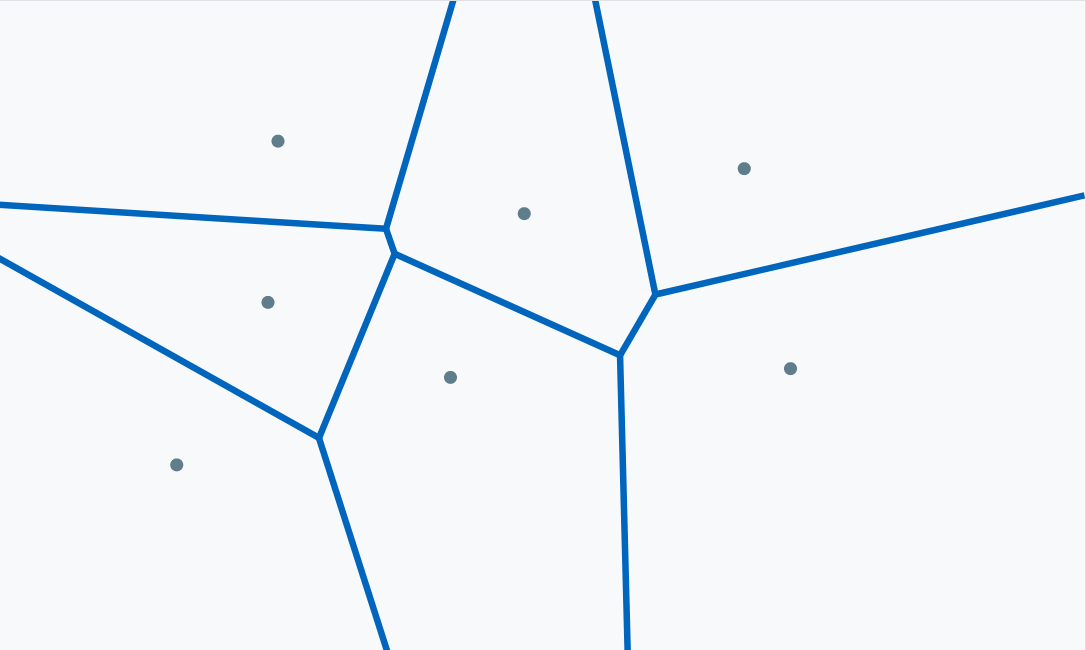
\includegraphics[width=.8\textwidth]{slidesRes/dual2.png}}};

  \begin{scope}[shift={(image.center)},scale=3.2]
    \draw[red,ultra thick] 
      (-.5,-.4) .. controls (-.5,1) and (.5, 1) .. (.5,-.4) 
      arc(0:-180:.15) 
      (.2,-.4) .. controls (.2,-.2) and (-.2,-.2) .. (-.2,-.4)
      arc(0:-180:.15) (-.4,-.4);
    \draw[red,ultra thick] (0,.2) circle(4pt);
  \end{scope}
\end{tikzpicture}
\end{center}
  \caption{No satisface ninguna hipótesis del teorema.}
\end{figure}

\end{frame}

%\begin{frame}\frametitle{Propiedad de la intersección genérica.}
%\begin{block}{Propiedad de la intersección genérica}
%  \(P\) tiene la propiedad de intersección genérica con \(M\) si  
%  para todo \(T\subset P\),
%  se cumple que
%  \(\setint(\bigcap V_{T} \cap M) = \setint(\bigcap V_{T}) \cap M\)
%  y
%  \(\bigcap V_{T} \cap M\) es vacía o
%  bien tiene dimensión \(d-\ell\) donde \(\ell = \dim(\bigcap V_T)\)
%\end{block}
%TODO: PONER DIBUJO
%\end{frame}
%
%\begin{frame}\frametitle{Propiedad de la bola cerrada.}
%
%\begin{block}{Propiedad de la bola cerrada}
%  \(P\) tiene la propiedad de la bola cerrada con \(M\) si
%  para todo \(Q\subset P\) con \(0\le \dim Q \le d\)
%  se tiene que \(\bigcap V_{Q,M}\) es vacía o una
%  bola cerrada de dimensión \(d-\dim Q\).
%\end{block}
%  
%TODO: PONER DIBUJO
%\end{frame}

\begin{frame}
  \begin{center}
  ¿Y si en vez de hacer crecer las bolas les damos un tamaño fijo?
  \end{center}
\end{frame}

\subsection{Complejo de \v{C}ech}

\begin{frame}\frametitle{Complejo de \v{C}ech}
  \begin{Definicion}[Complejo de \v{C}ech]
  El complejo de \v{C}ech a escala \(\epsilon\) se define por: 
  \begin{align*}
    Q \in \Cech(P,\epsilon)
    \text{ si y solo si }
    \bigcap_{q\in Q} B(q,\epsilon) \ne \varnothing. 
  \end{align*}
  \end{Definicion}

  \begin{figure}[H]
  \begin{columns}
    \column{.6\linewidth}
    \centering
    \fbox{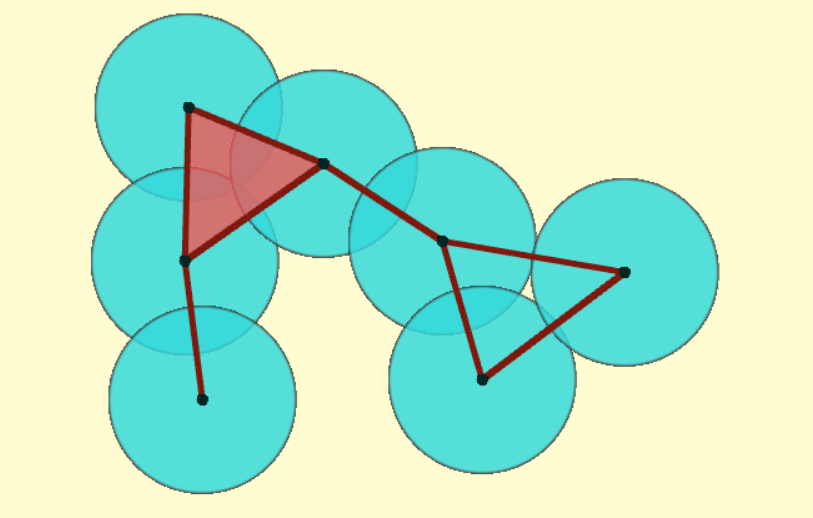
\includegraphics[width=.8\textwidth]{slidesRes/cech.png}}
    \column{.3\linewidth}
    \caption{Complejo de \v{C}ech de 7 puntos en el plano.}
  \end{columns}
  \end{figure}
\end{frame}

\begin{frame}\frametitle{¿Cómo reconstruye \v{C}ech?}
  %\begin{block}{Observación}
  %  \(\Cech(P,\epsilon)\) se puede caracterizar como
  %  \begin{displaymath}
  %    \nerve C
  %    \coloneqq
  %    \left\{ 
  %    D\subset C\colon \bigcap D \ne \varnothing.
  %    \right\} 
  %  \end{displaymath}
  %  donde \(C = \bigcup_{p\in P} B(p,\epsilon)\). 
  %\end{block}

  \begin{Teorema}[Nervio]
    \(\Cech(P,\epsilon)\) es homotópicamente equivalente%
    \footnote[frame]{\(X\) y \(Y\) son homotópicamente equivalentes si existen
    funciones continuas \(f\colon X \to Y\) y \(g\colon Y \to X\)
    tales que \(f\circ g \sim id_Y\) y \(g\circ f \sim id_X\)}
    a \(\bigcup_{p\in P} B(p,\epsilon) = P^{\oplus\epsilon}\).  
  \end{Teorema}

\end{frame}

\begin{frame}\frametitle{¿Cómo reconstruye \v{C}ech?}
  \begin{Teorema}[Niyogi, P., Smale, S., Weinberger, S. (2008)]
    Si \(P\) es una muestra \(\epsilon/2\)-densa \(0\)-ruidosa de \(M\)
    y \(\epsilon < \sqrt{3/5}\, \RR\) entonces 
    \(P^{\oplus\epsilon}\) y \(M\) son homotópicamente equivalentes.
  \end{Teorema}
  \begin{columns}
    \column{.45\textwidth}
    \centering\fbox{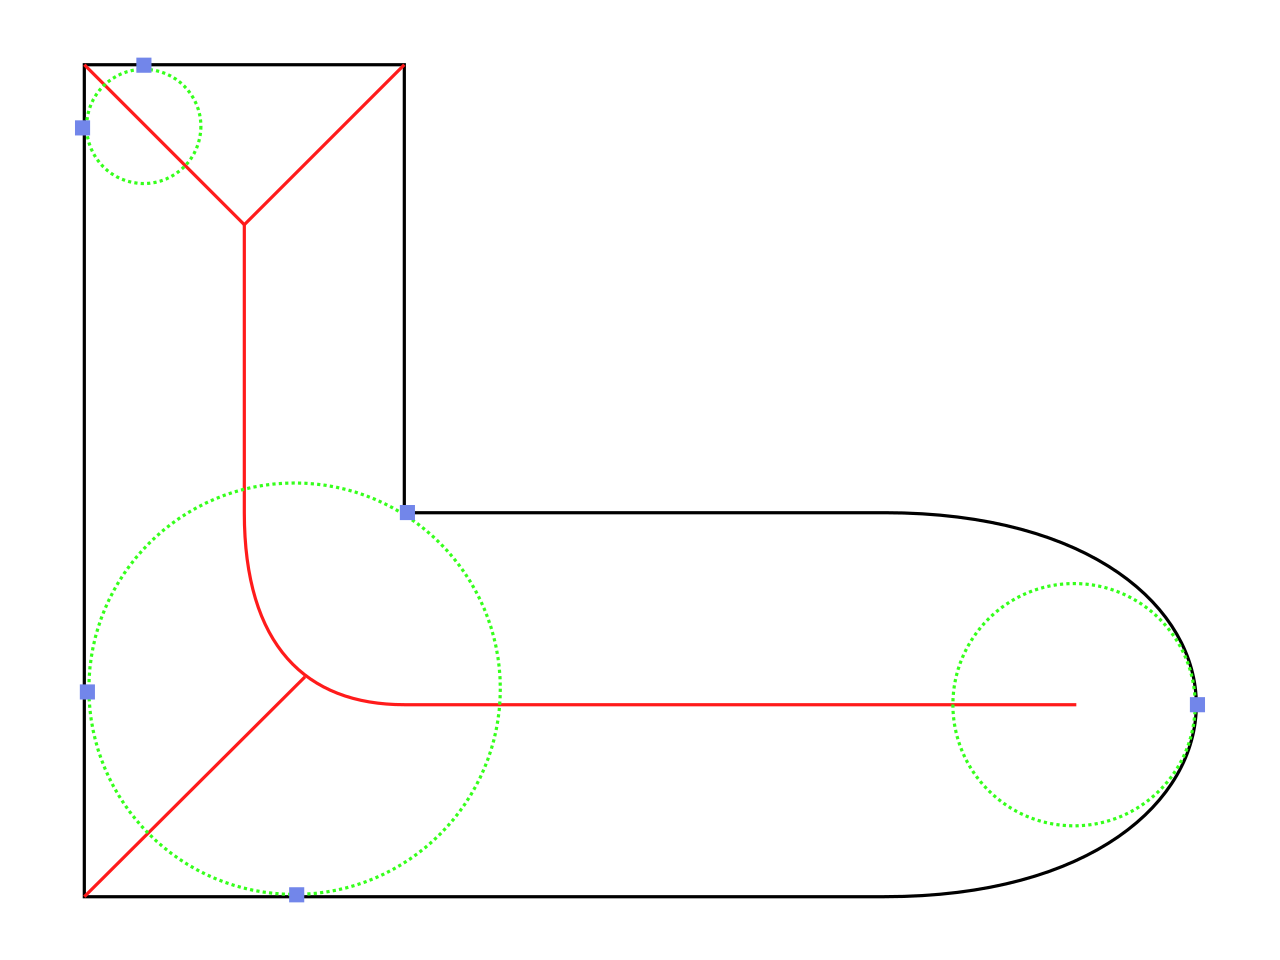
\includegraphics[width=\textwidth]{slidesRes/medial_axis.png}}
    \column{.5\textwidth}
    El alcance de un conjunto \(X\) es 
    \[ 
      \RR \coloneqq \inf_{x\in X} d(x, \medialAxis(X))
    \]
    donde \(\medialAxis(X)\) son los \(y\in \R^N\) que
    tienen al menos 2 puntos más cercanos a \(X\). 
  \end{columns}
\end{frame}

\begin{frame}
\begin{center}
  ¿Podemos relajar las condiciones?
\end{center} 
\end{frame}

\subsection{Complejo de Rips}

\begin{frame}\frametitle{Complejo de Rips}
  \begin{Definicion}[Complejo de Rips]
  El complejo de Vietoris-Rips a escala \(\epsilon\) se define por: 
    \begin{equation*}
      Q\in \VR(P,\epsilon) 
      \text{ si y solo si }
      \diam Q \le \epsilon.
    \end{equation*}
  \end{Definicion}

  \begin{figure}[H]
    \begin{columns}
    \column{0.7\linewidth}
    \centering\fbox{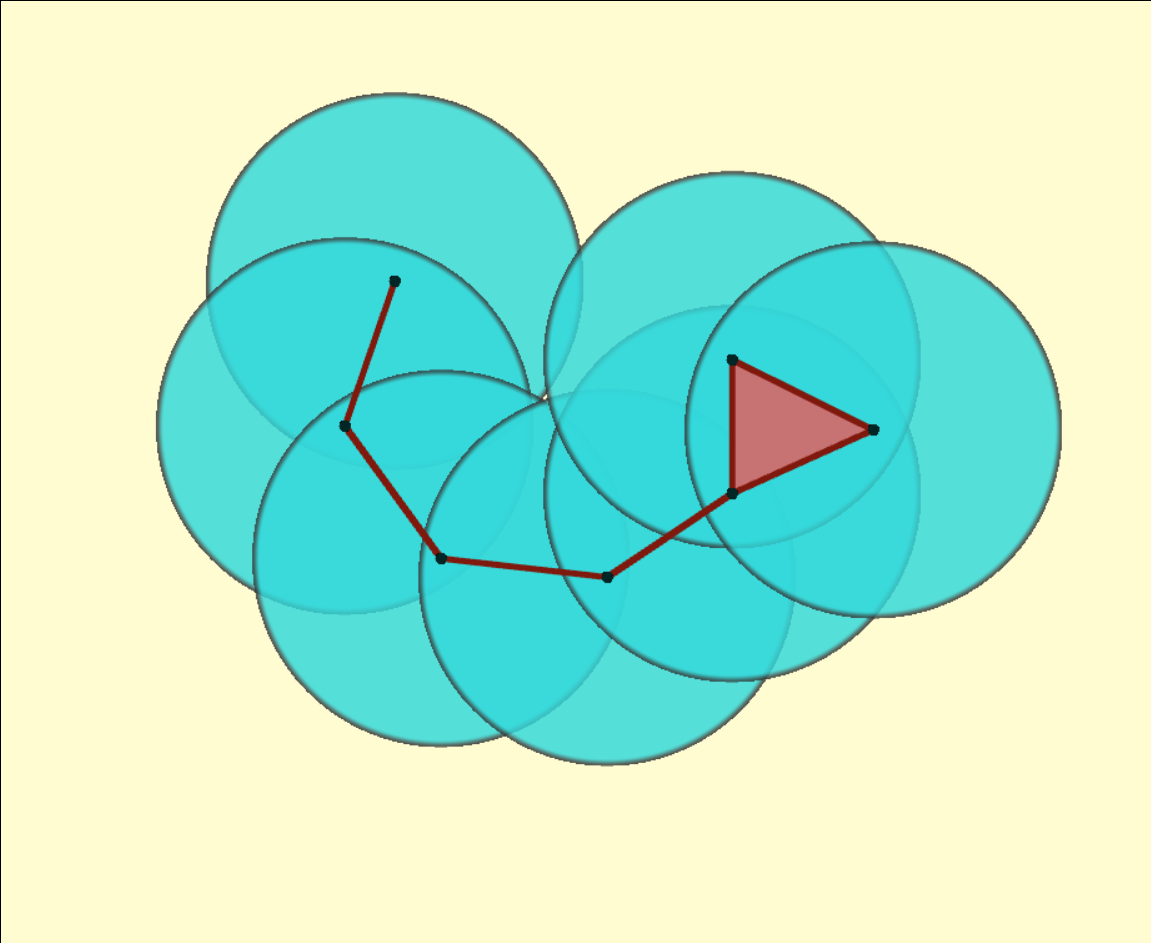
\includegraphics[width=0.7\textwidth]{slidesRes/rips.png}}
    \column{0.3\linewidth}
    \caption{El complejo de Rips de 7 puntos en el plano.}
    \end{columns}
  \end{figure}

\end{frame}

\begin{frame}\frametitle{Observaciones}
\begin{columns}
  \column{.7\linewidth}
  \begin{itemize}
    \item<1-> El complejo está determinado por sus aristas.
    \begin{center}
    \begin{tikzpicture}[scale=1, transform shape]
      \node[myvertex] (A) at (-.5,0) {};
      \node[myvertex] (B) at (.5,0) {};
      \node[myvertex] (C) at (0,1) {};
      \draw[myedge] (A) -- (B) -- (C) -- (A);
    \end{tikzpicture}
    \end{center}
    
    \item<2-> Solo se requiere información espacial para computar las aristas
      el resto es combinatorial.
  \end{itemize}

  \column{.3\linewidth}
  \begin{figure}[H]
    \begin{overprint}
    \onslide<1>
      \centering\fbox{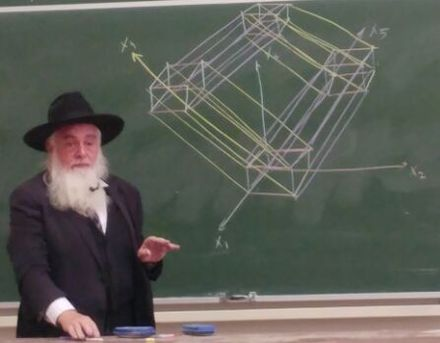
\includegraphics[width=\textwidth]{slidesRes/eliyahu-rips.jpg}}
      \caption{Eliyahu Rips. Matemático Israelí.}
    \onslide<2> 
      \centering\fbox{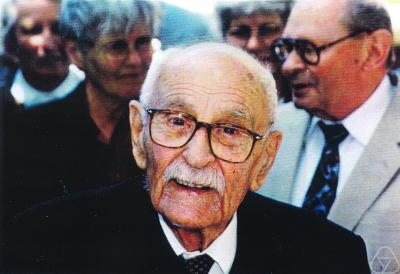
\includegraphics[width=\textwidth]{slidesRes/leopold-vietoris.jpg}}
      \caption{Leopold Vietoris. Matemático Austro-Húngaro.}
    \end{overprint}
  \end{figure}
\end{columns}
\end{frame}

\begin{frame}
  \begin{center}
    ¿Qué tanto se parece \v{C}ech y Rips?
  \end{center}
\end{frame}

\begin{frame}\frametitle{Relación entre \v{C}ech y Rips.}
  \begin{overprint}
  \onslide<1>
  \begin{columns}
    \column{.5\linewidth}
    \begin{figure}[H]
      \centering\fbox{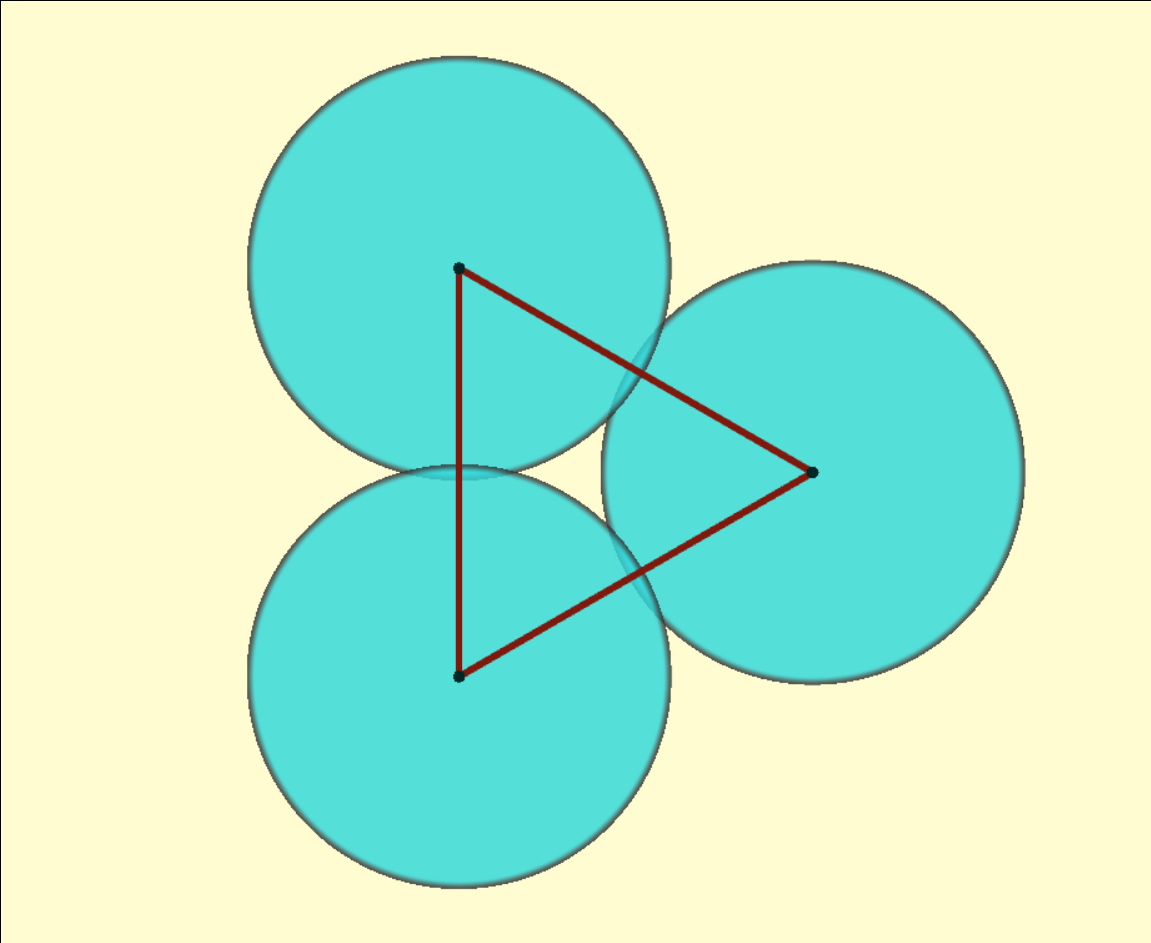
\includegraphics[width=\textwidth]{slidesRes/cech_045_rips.png}}
      \caption{\(\Cech(P, 0.45)\)}
    \end{figure}

    \column{.5\linewidth}
    \begin{figure}[H]
      \centering\fbox{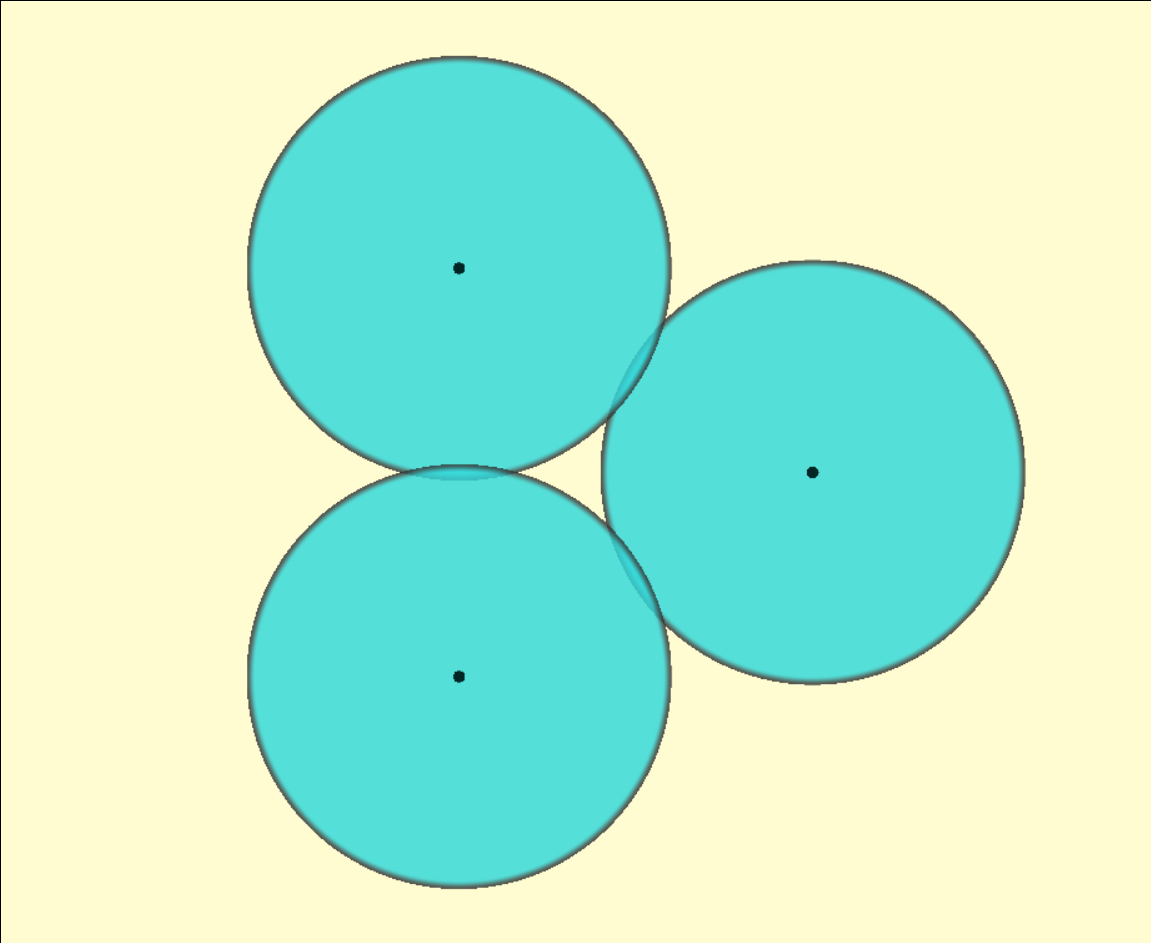
\includegraphics[width=\textwidth]{slidesRes/cech_rips_045.png}}
      \caption{\(\VR(P, 0.45)\)}
    \end{figure}
  \end{columns}

  \onslide<2>
  \begin{columns}
    \column{.5\linewidth}
    \begin{figure}[H]
      \centering\fbox{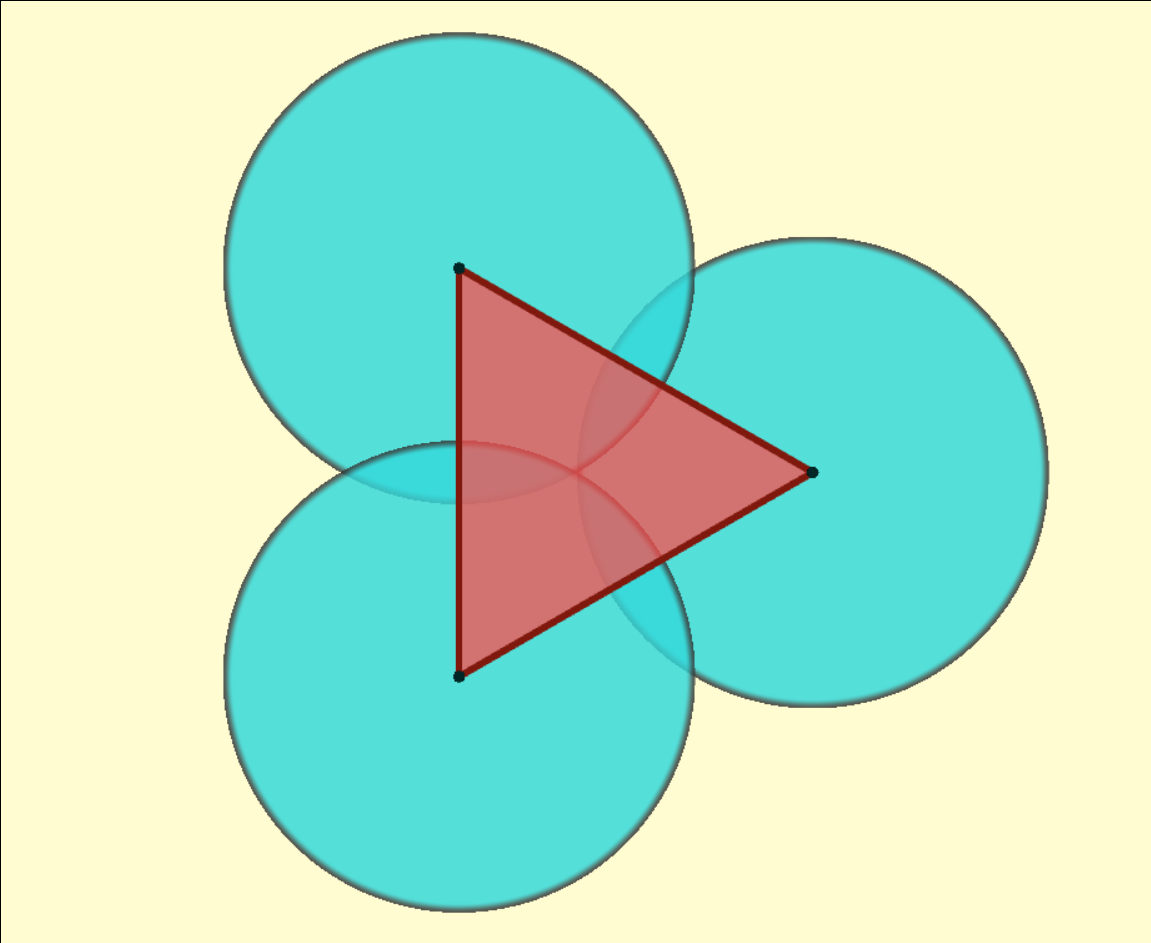
\includegraphics[width=\textwidth]{slidesRes/cech_05_rips.png}}
      \caption{\(\Cech(P, 0.5)\)}
    \end{figure}

    \column{.5\linewidth}
    \begin{figure}[H]
      \centering\fbox{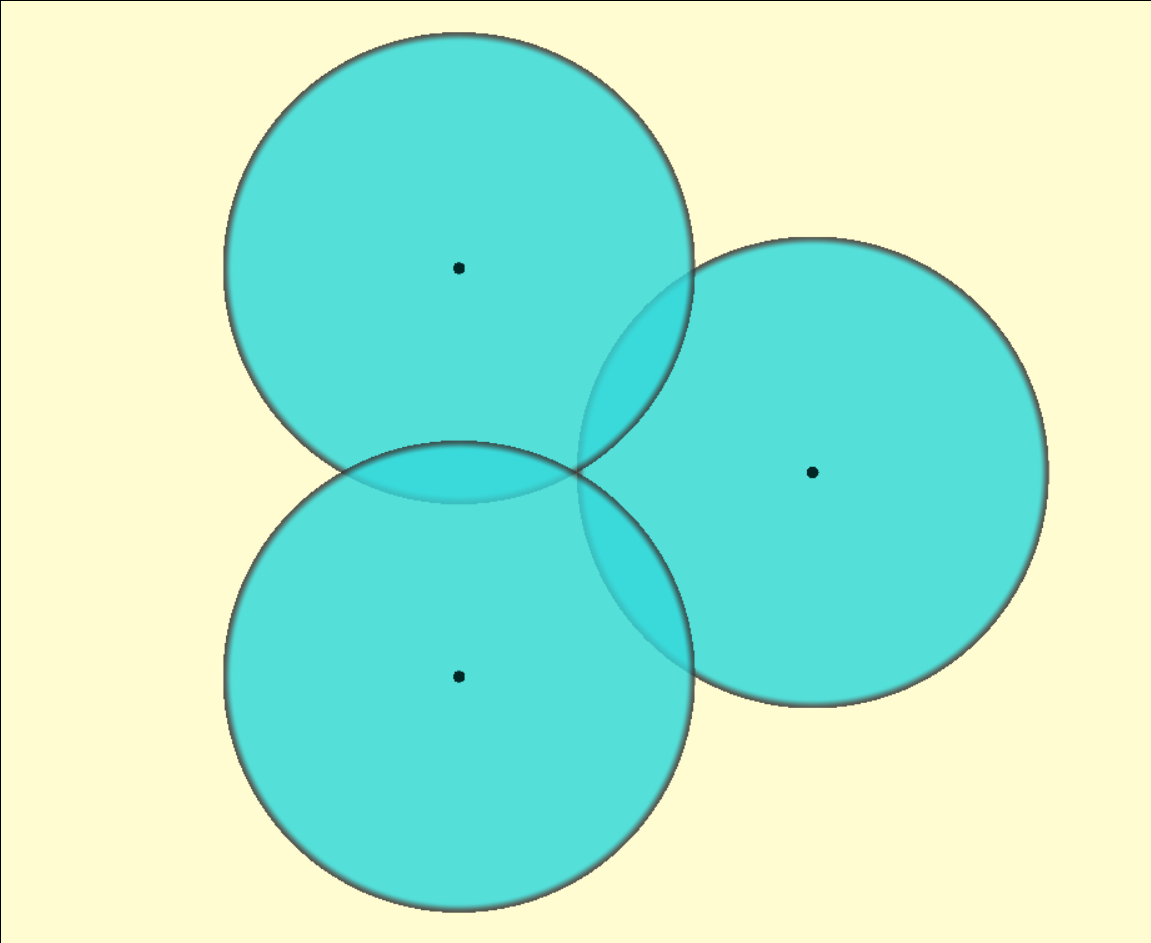
\includegraphics[width=\textwidth]{slidesRes/cech_rips_05.png}}
      \caption{\(\VR(P, 0.5)\)}
    \end{figure}
  \end{columns}

  \onslide<3>
  \begin{columns}
    \column{.5\linewidth}
    \begin{figure}[H]
      \centering\fbox{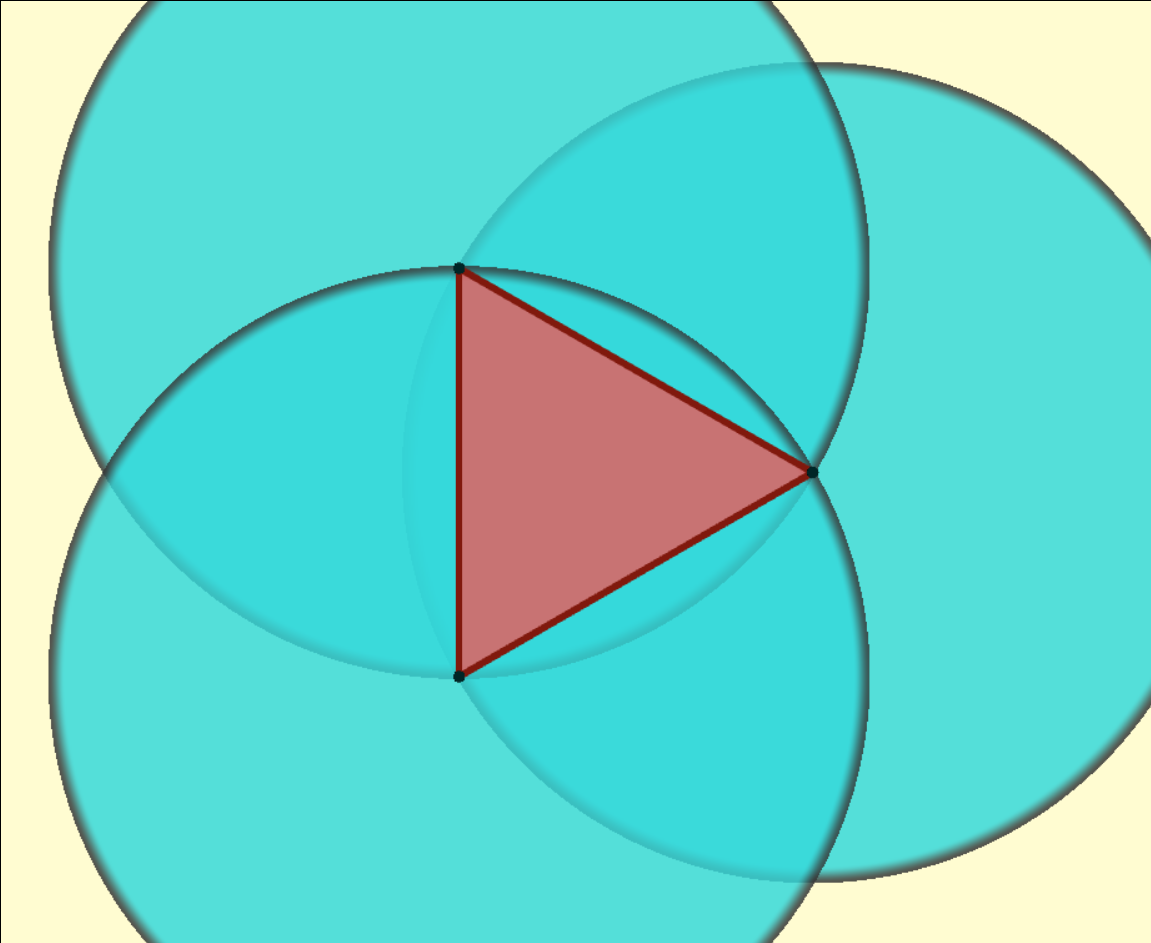
\includegraphics[width=\textwidth]{slidesRes/cech_087_rips.png}}
      \caption{\(\Cech(P, 0.87)\)}
    \end{figure}

    \column{.5\linewidth}
    \begin{figure}[H]
      \centering\fbox{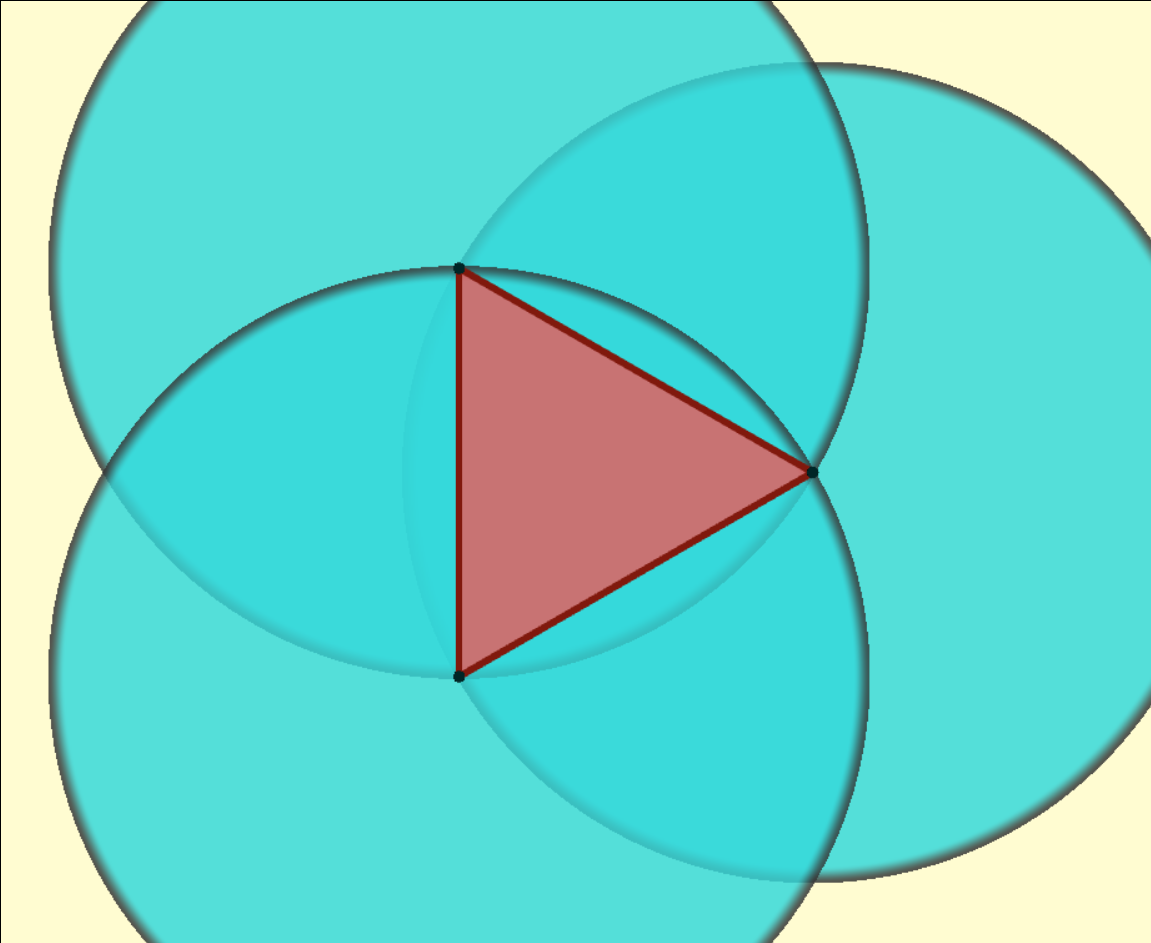
\includegraphics[width=\textwidth]{slidesRes/cech_rips_087.png}}
      \caption{\(\VR(P, 0.87)\)}
    \end{figure}
  \end{columns}
  \end{overprint}
\end{frame}

\begin{frame}\frametitle{Relación entre \v{C}ech y Rips.}
  \begin{Proposicion}[a veces, Rips se parece a \v{C}ech]
  \begin{displaymath}
    \Cech(P,\epsilon) \subset \VR(P,2\epsilon) \subset \Cech(P,2 \epsilon \rho_N)
  \end{displaymath}
  donde \(\rho_N \coloneqq \sqrt{\frac{2N}{N+1}}\).
  \end{Proposicion}
\end{frame}

%%%%%%%%%%%%%%%%%%%%%%%%%%%%%%%%%%%%%%%%%%%%%%%%%%%%%%%%%%%%%%%%%
\section{Algoritmos}

\begin{frame}\frametitle{Observaciones}
  Antes de crear un algoritmo debemos establecer la interfaz:
  \begin{itemize}
    \item La entrada son puntos en posición general y un parámetro de escala.
    \item La salida son los símplices maximales.
  \end{itemize}
\end{frame}

\subsection{Complejo de \v{C}ech}

\begin{frame}\frametitle{Computar el Complejo de \v{C}ech}
\begin{columns}
  \column{.7\textwidth}
  \begin{block}{Observación}
    \(Q\in \Cech(P,\epsilon)\) si y solo sí la bola de cobertura mínima de 
    \(Q\) tiene radio menor a \(\epsilon\). 
  \end{block}

  \begin{center}
  \fbox{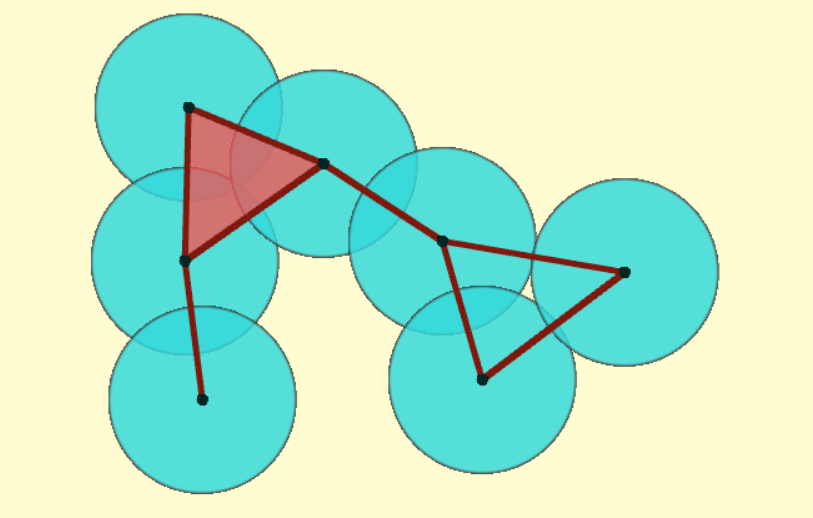
\includegraphics[width=.7\textheight]{slidesRes/cech.png}}
  \end{center}

  \column{.25\textwidth}
  \begin{figure}[H]
    \centering
    \fbox{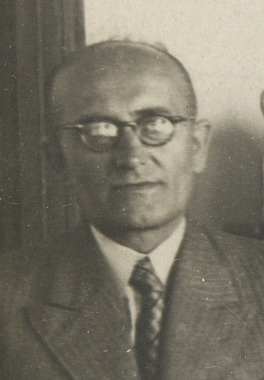
\includegraphics[width=\textwidth]{slidesRes/eduard-cech.jpg}}
    \caption{Eduard \v{C}ech. Matemático Austro-Húngaro.}
  \end{figure}
\end{columns}
\end{frame}

\begin{frame}\frametitle{Computar el Complejo de \v{C}ech}
\begin{block}{Idea}
  Buscar todas las posibles bolas de cobertura mínima de radio menor a \(\epsilon\).
\end{block}

\pause%
¿Complejidad? hay que buscar la bola de cobertura mínima en cada dimensión:
\begin{displaymath}
  \sum_{k=1}^{N+1} {n\choose k}
  =
  \sum_{k=1}^{N+1} \OO(n^k)
  \le
  \OO((N+1)\, n^{N+1})
\end{displaymath}

\pause%
¿Cuánto toma computar la bola de cobertura mínima?
\end{frame}

\begin{frame}\frametitle{Bola de Cobertura Mínima}

\begin{columns}
  \column{.6\textwidth}
  \begin{Definicion}[Bola de Cobertura Mínima]
  La bola de cobertura mínima, \(MB(P)\), 
  es la bola de menor radio tal que \(P\subset MB(P)\).
  \end{Definicion}

  Observaciones:
  \begin{itemize}
    \item \(MB(P)\) existe y es única.
    \item \(MB(P)\) está determinada por a lo más \(N+1\) puntos de \(P\).  
  \end{itemize}

  \column{.35\textwidth}
  \begin{figure}[H]
    \centering
    \fbox{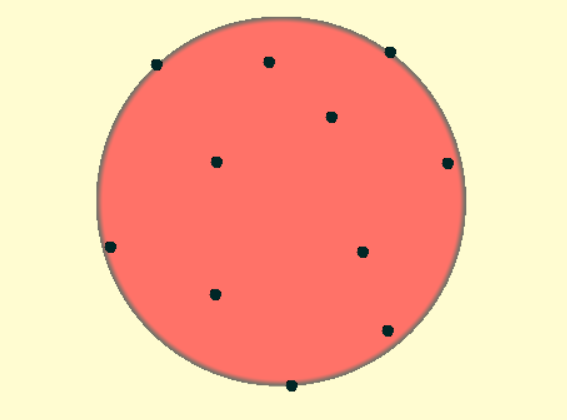
\includegraphics[width=\textwidth]{slidesRes/seb.png}}
    \caption{Bola de Cobertura Mínima de 11 puntos en el plano.}
  \end{figure}
\end{columns}
\end{frame}

\begin{frame}\frametitle{Algoritmo de Welzl}
\begin{columns}
  \column{.7\linewidth}
  \begin{Algoritmo}
  \Function{MinBall}{P,S}
    \If{\(P=\varnothing\) or \(\card S = N+1\)}
      \State{\Return{SphereThrough(S)}}
    \EndIf%
    \State{\textbf{pick} \(p\in P\)}
    \State{\(B \gets \Call{MinBall}{P-p, S}\)}
    \If{\(p\in B\)}
      \State{\Return{\(B\)}}
    \EndIf
    \State{\Return{\(\Call{MinBall}{P-p, S+p}\)}}
  \EndFunction%
  \end{Algoritmo}

  ¿Complejidad? Caso esperado de \(\OO(n)\), pero peor caso de \(\OO(n^3)\).

  \column{.25\linewidth}
  \begin{figure}[H]
    \centering
    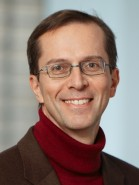
\includegraphics[width=\textwidth]{slidesRes/emo-welzl.jpeg}
    \caption{Emo Welzl. Científico Computacional Austriaco.}
  \end{figure}
\end{columns}

\end{frame}

%\begin{frame}
%\begin{Proposicion}
%\begin{itemize}
%  \item Si \(\card S = N+1\), entonces \(MB(S)\) es la única bola que
%  circumbscribe a \(S\).
%  \item Si \(\card S < N+1\), todos los candidatos a centro de \(MB(S)\) residen
%  en el espacio ortogonal a \(\aff(S)\) que pasa por \(\centre MB(S)\).  
%\end{itemize}
%\end{Proposicion}
%
%\begin{proof}
%  Sea \(S = \left\{ S_0, \ldots, S_k \right\} \) y
%  \(x\coloneqq \centre(MB(S))\). Luego, \(x\) resuelve el sistema \(Ax = b\) donde 
%  \begin{displaymath}
%    A =
%    \begin{bmatrix}
%      (S_1 - S_0)^T\\
%      \vdots\\
%      (S_k - S_0)^T\\
%      \end{bmatrix}
%    \qquad\text{y}\qquad
%    b =
%    \frac{1}{2}
%    \begin{pmatrix}
%      \norm{S_1}^2 - \norm{S_0}^2\\
%      \vdots\\
%      \norm{S_k}^2 - \norm{S_0}^2
%    \end{pmatrix}
%  \end{displaymath}
%  Si \(k=N\) el sistema tiene solución única. Si \(k<N\) entonces
%  \begin{displaymath}
%    y\in \ker A \iff y \perp \aff(S)
%    \Rightarrow
%    A(x-y) = b
%  \end{displaymath}
%\end{proof}
%\end{frame}

\begin{frame}\frametitle{Computar el Complejo de \v{C}ech}
  Computar todo el complejo de \v{C}ech debería tomar \(\OO( (N+1)\, n^{N+4})\)

  \pause
  Recordar debemos retornar sólo los símplices maximales.
  \begin{itemize}
    \item Podemos verificar que los símplices más chicos no estén en símplices más grandes (Top-Down).
    \item {\bfseries Podemos construir los símplices más grandes a partir de los símplices más chicos (Bottom-up).}
  \end{itemize}
\end{frame}

\begin{frame}\frametitle{Computar el Complejo de \v{C}ech}
\begin{Algoritmo}
  \Function{computeCechSkeleton}{P,\(\epsilon\),dim}
    \State{\(L \gets P \)}
    \For{\(d\gets 1,\ldots, dim\)}
      \State{\(H \gets \varnothing\)}
      \For{each simplex \(\sigma \in L\) of \(\dim \sigma = d-1\)}
        \For{each \(p\in P\) not in \(\sigma\)}
          \If{radius of \(MB(\sigma\cup \lbrace p \rbrace) < \epsilon\)}
            \State{\(H\gets H \cup \lbrace \sigma \cup \lbrace p \rbrace \rbrace\) }
          \EndIf%
        \EndFor%
      \EndFor%
      \State{\(H\gets H\,\cup \) simplices in \(L\) that weren't previously merged}
      \State{\(L\gets H\)}
    \EndFor%
    \State{\Return{\(L\)}}
  \EndFunction%
\end{Algoritmo}

  ¿Complejidad? Peor caso de \(\OO(dim\cdot n^{dim+4})\). 
\end{frame}

\subsection{Complejo de Rips}

\begin{frame}\frametitle{Computar el Complejo de Rips}
  \begin{Algoritmo}
  \Function{computeRipsSkeleton}{P,\(\epsilon\),dim}
    \State{\(L \gets P \)}
    \For{\(d\gets 1,\ldots, dim\)}
      \State{\(H \gets \varnothing\)}
      \For{each simplex \(\sigma \in L\) of \(\dim \sigma = d-1\)}
        \For{each \(p\in P\) not in \(\sigma\)}
          \If{\(\diam(\sigma\cup \lbrace p \rbrace) < \epsilon\)}
            \State{\(H\gets H \cup \lbrace \sigma \cup \lbrace p \rbrace \rbrace\) }
          \EndIf%
        \EndFor%
      \EndFor%
      \State{\(H\gets H\,\cup \) simplices in \(L\) that weren't previously merged}
      \State{\(L\gets H\)}
    \EndFor%
    \State{\Return{\(L\)}}
  \EndFunction%
  \end{Algoritmo}

  ¿Complejidad? Peor caso de \(\OO(dim^2\cdot n^{dim+1})\). 
\end{frame}

\begin{frame}\frametitle{Fin}
  \centering\fbox{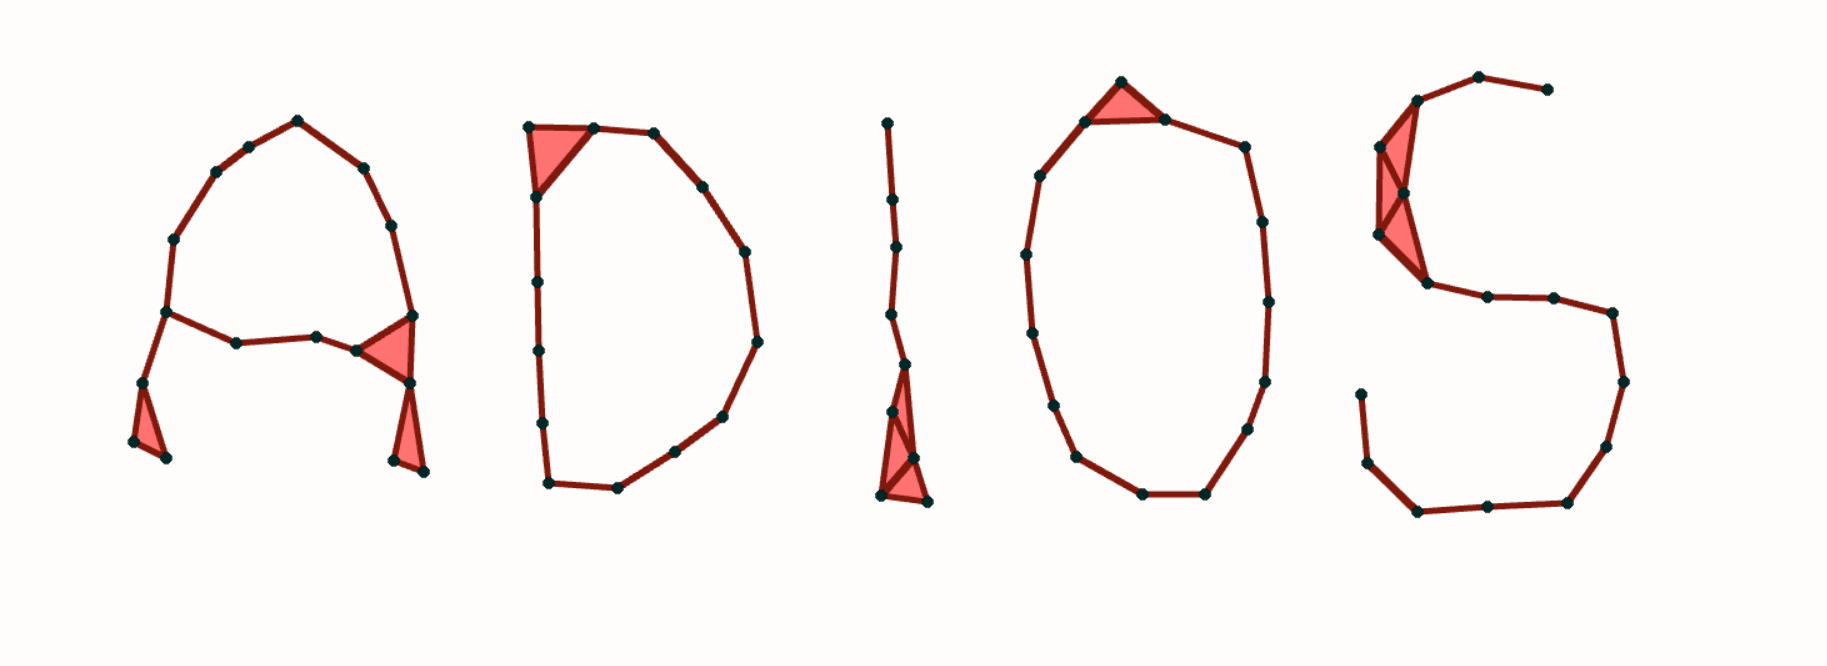
\includegraphics[width=0.8\textwidth]{slidesRes/adios2.png}}
\end{frame}

\begin{frame}\frametitle{Referencias}
  
\begin{thebibliography}{9}
\bibitem{coverage}
De Silva, V., \& Ghrist, R. (2007). Coverage in sensor networks via persistent homology. Algebraic \& Geometric Topology, 7(1), 339-358.

\bibitem{triangulating}
Edelsbrunner, H., \& Shah, N. R. (1994, June). Triangulating topological spaces. In Proceedings of the tenth annual symposium on Computational geometry (pp. 285-292).

\bibitem{retracto}
Niyogi, P., Smale, S., Weinberger, S. (2008). Finding the homology of submanifolds with high confidence from random samples. Discrete \& Computational Geometry, 39, 419-441.

\bibitem{welzl}
Welzl, E. (2005, June). Smallest enclosing disks (balls and ellipsoids). In New Results and New Trends in Computer Science: Graz, Austria, June 20–21, 1991 Proceedings (pp. 359-370). Berlin, Heidelberg: Springer Berlin Heidelberg.

\bibitem{cechconstruction}
Dantchev, S., \& Ivrissimtzis, I. (2012). Efficient construction of the Čech complex. Computers \& graphics, 36(6), 708-713.
\end{thebibliography}
\end{frame}

\end{document}
